% Created 2021-05-31 Mon 12:20
% Intended LaTeX compiler: pdflatex
\documentclass[10pt]{article}
     \usepackage{/home/john/texstuff/NoTeX/NotesTeXSW}
     \input{/home/john/skola/test/test3/bold.tex}
     \usepackage{minted}
\date{\today}
\title{Project 1 MM5016}
\hypersetup{
 pdfauthor={},
 pdftitle={Project 1 MM5016},
 pdfkeywords={},
 pdfsubject={},
 pdfcreator={Emacs 27.2 (Org mode 9.4.4)}, 
 pdflang={Samin}}
\begin{document}

\maketitle

\section{Introduction}
\label{sec:org82166b2}
In this document, 4 numerical methods for solving a specific ODE
will be visualised and briefly discussed. The numerical methods being:
Euler's method, second order Runge-Kutta, fourth order Runge-Kutta and the
Adam-Basforth method. The ODE that these methods will try to approximate will
be the solution to:
\begin{align*}
\frac{du}{dt} = \cos(\pi t) + u(t)
,
\end{align*}

with initial value \(u(0) = 2\). The analytical solution can
be yielded by mutliplying with an integrating factor as such:
\begin{align*}
 &  \frac{du}{dt} = \cos (\pi t) + u(t) \\
\implies & \frac{du}{dt} - u(t) = \cos(\pi t) \\
\implies & e^{-t} \frac{du}{dt} - e^{-t} u(t) = e^{-t} \cos(\pi t) \\
\implies & \frac{d}{dt} ( e^{-t} u (t)) = e^{-t} \cos( \pi t ) \\
\implies & e^{-t} u(t) = C + \int_{  } e^{-t} \cos (\pi t) dt \\
\implies & u(t) = e^{t} C + e^{t} \int_{  } e^{-t} \cos (\pi t) dt 
.
\end{align*}

The integral on the right can be evaluated using repeated partial integration,
so an analytical solution exists, and it will be the one we will compare with
the approximated solutions from the numerical methods.


All the following graphs can be generated by running the included python 3 scripts in a terminal.
\newpage
\section{Graphs}
\label{sec:orgb8ee4e1}

\subsection{Euler's method}
\label{sec:org35a2f47}
\begin{center}
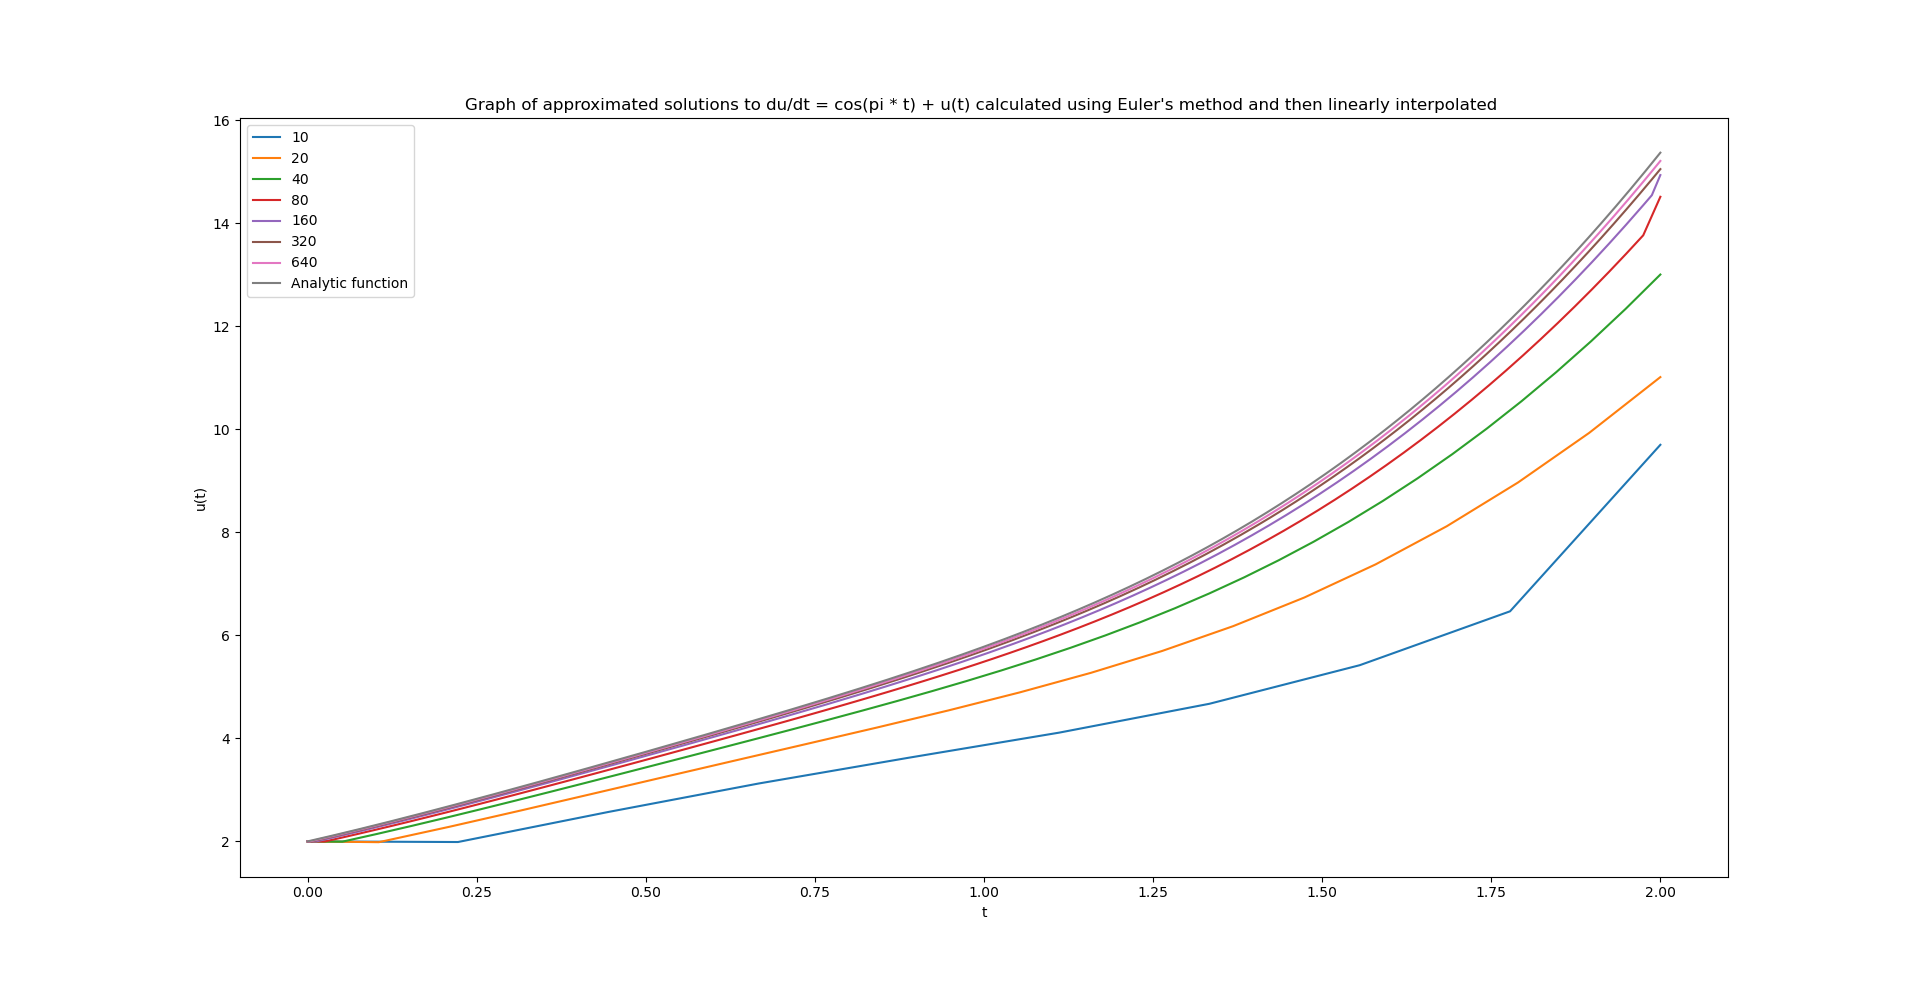
\includegraphics[angle=0,height=10cm]{./img/euler_function.png}
\end{center}

\begin{center}
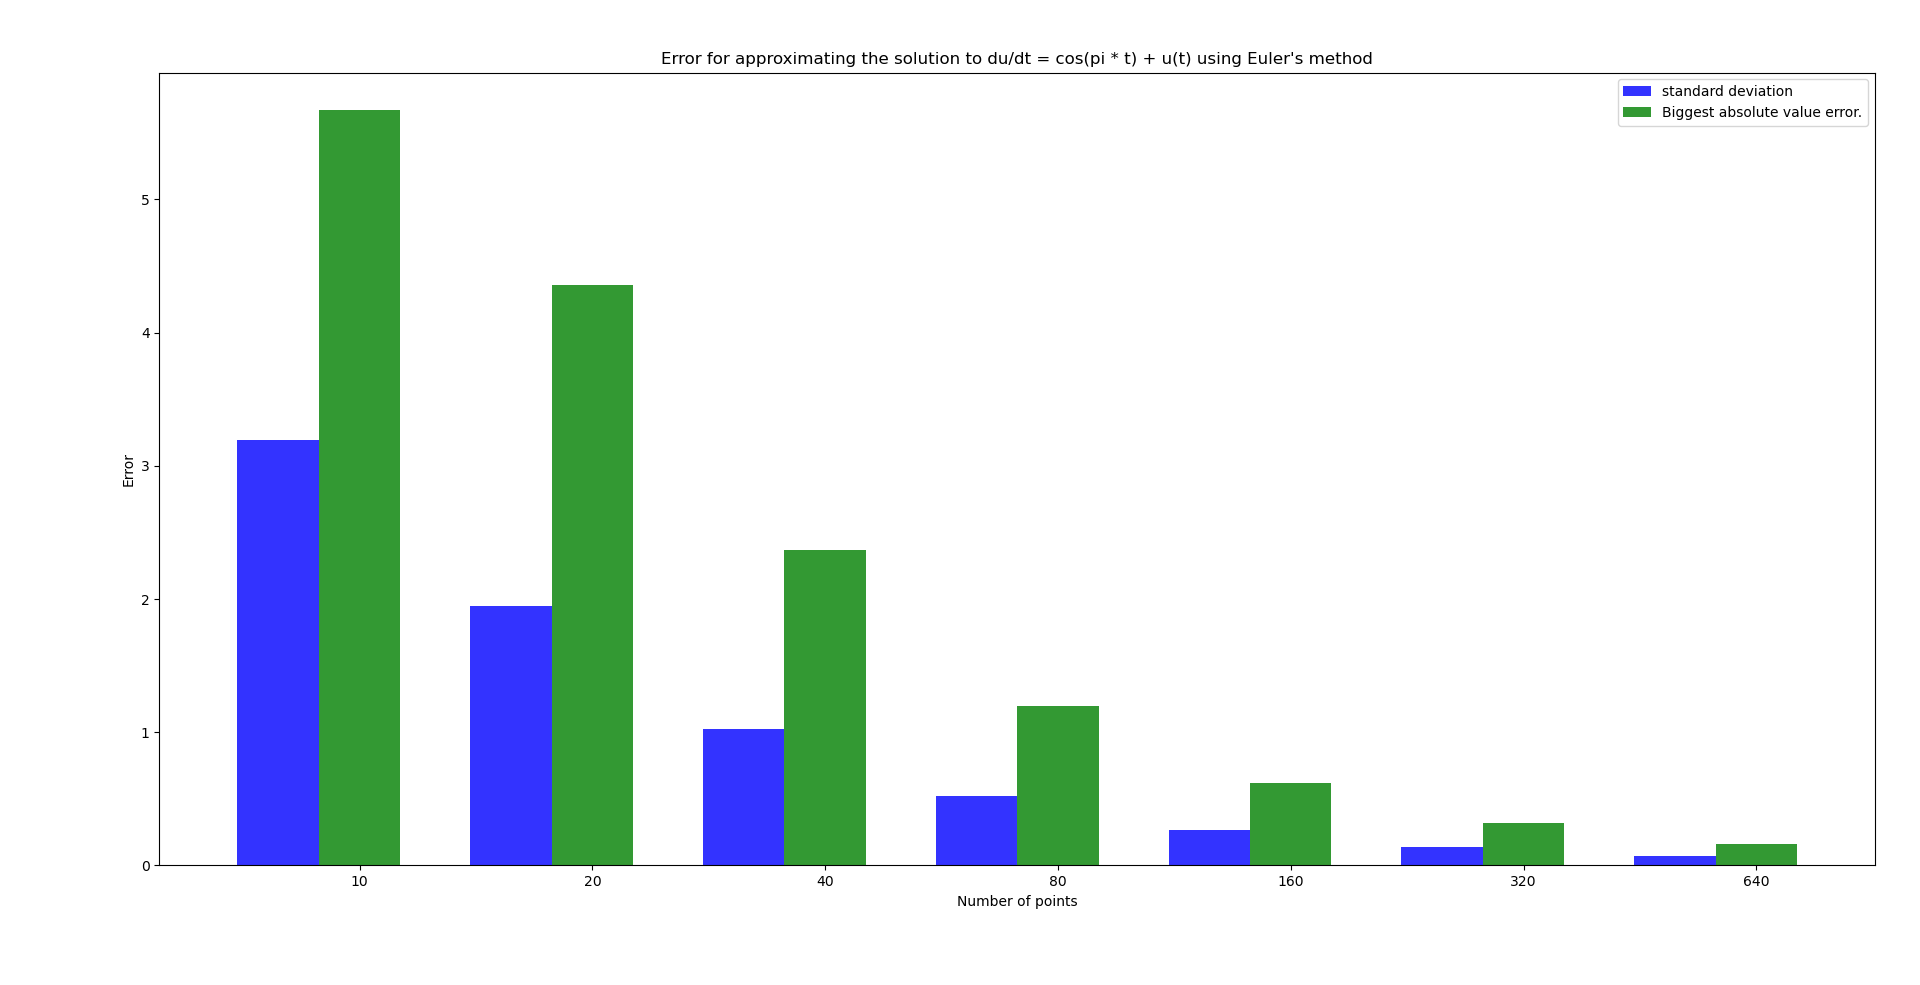
\includegraphics[angle=0,height=10cm]{./img/euler_error.png}
\end{center}


\subsection{2nd order Runge Kutta}
\label{sec:orgd8b3b71}

\begin{center}
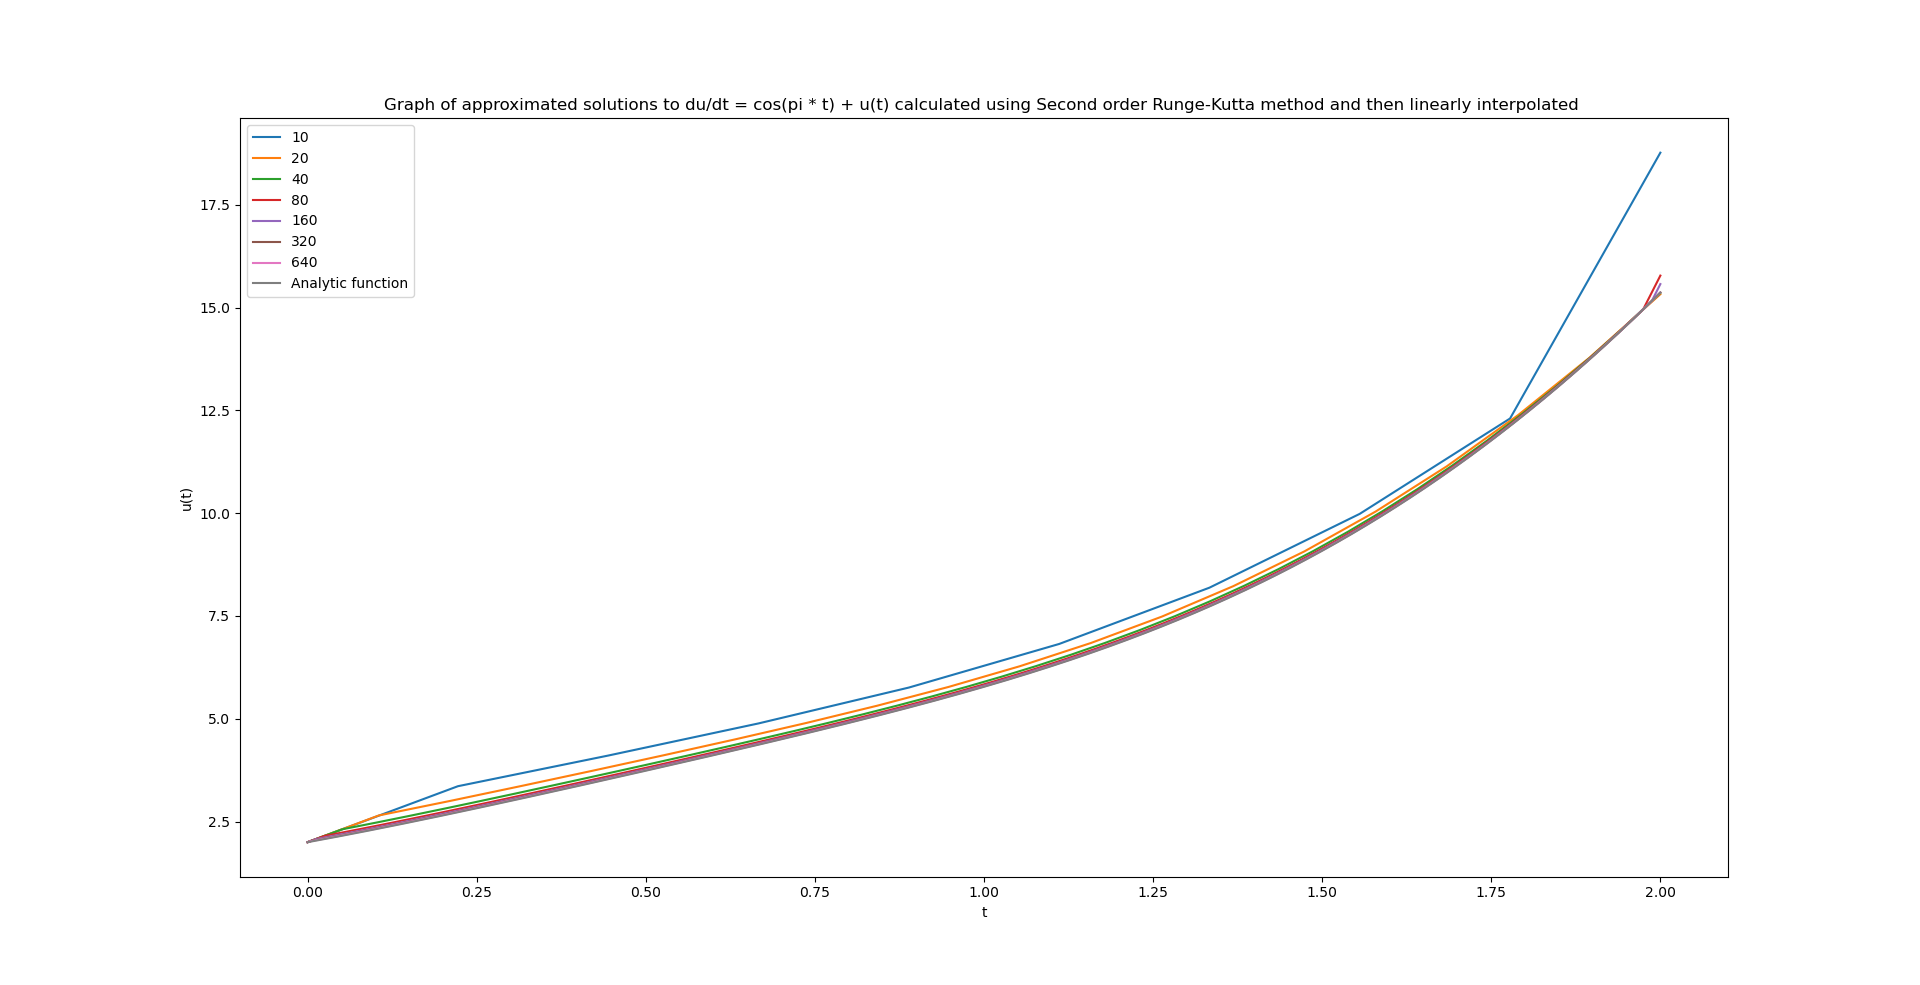
\includegraphics[angle=0,height=10cm]{./img/runge_2_function.png}
\end{center}

\begin{center}
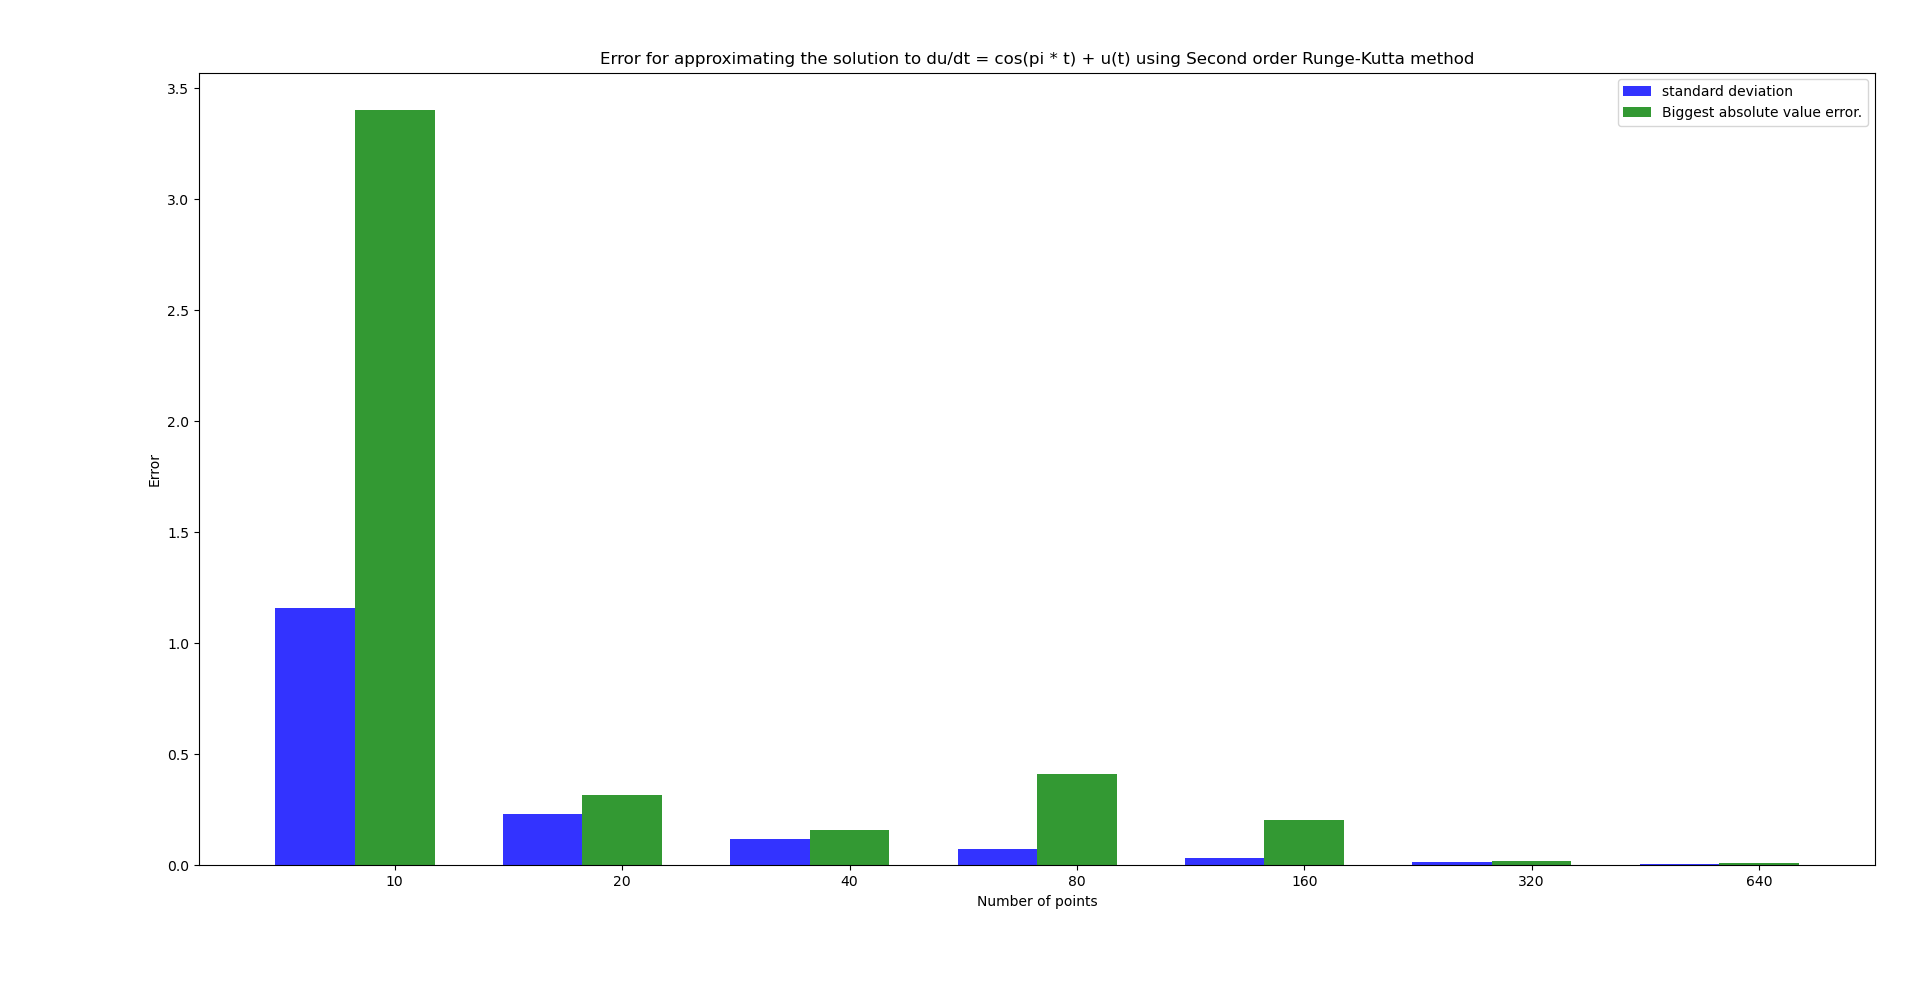
\includegraphics[angle=0,height=10cm]{./img/runge_2_error.png}
\end{center}




\subsection{4th order Runge Kutta}
\label{sec:orgd94704c}

\begin{center}
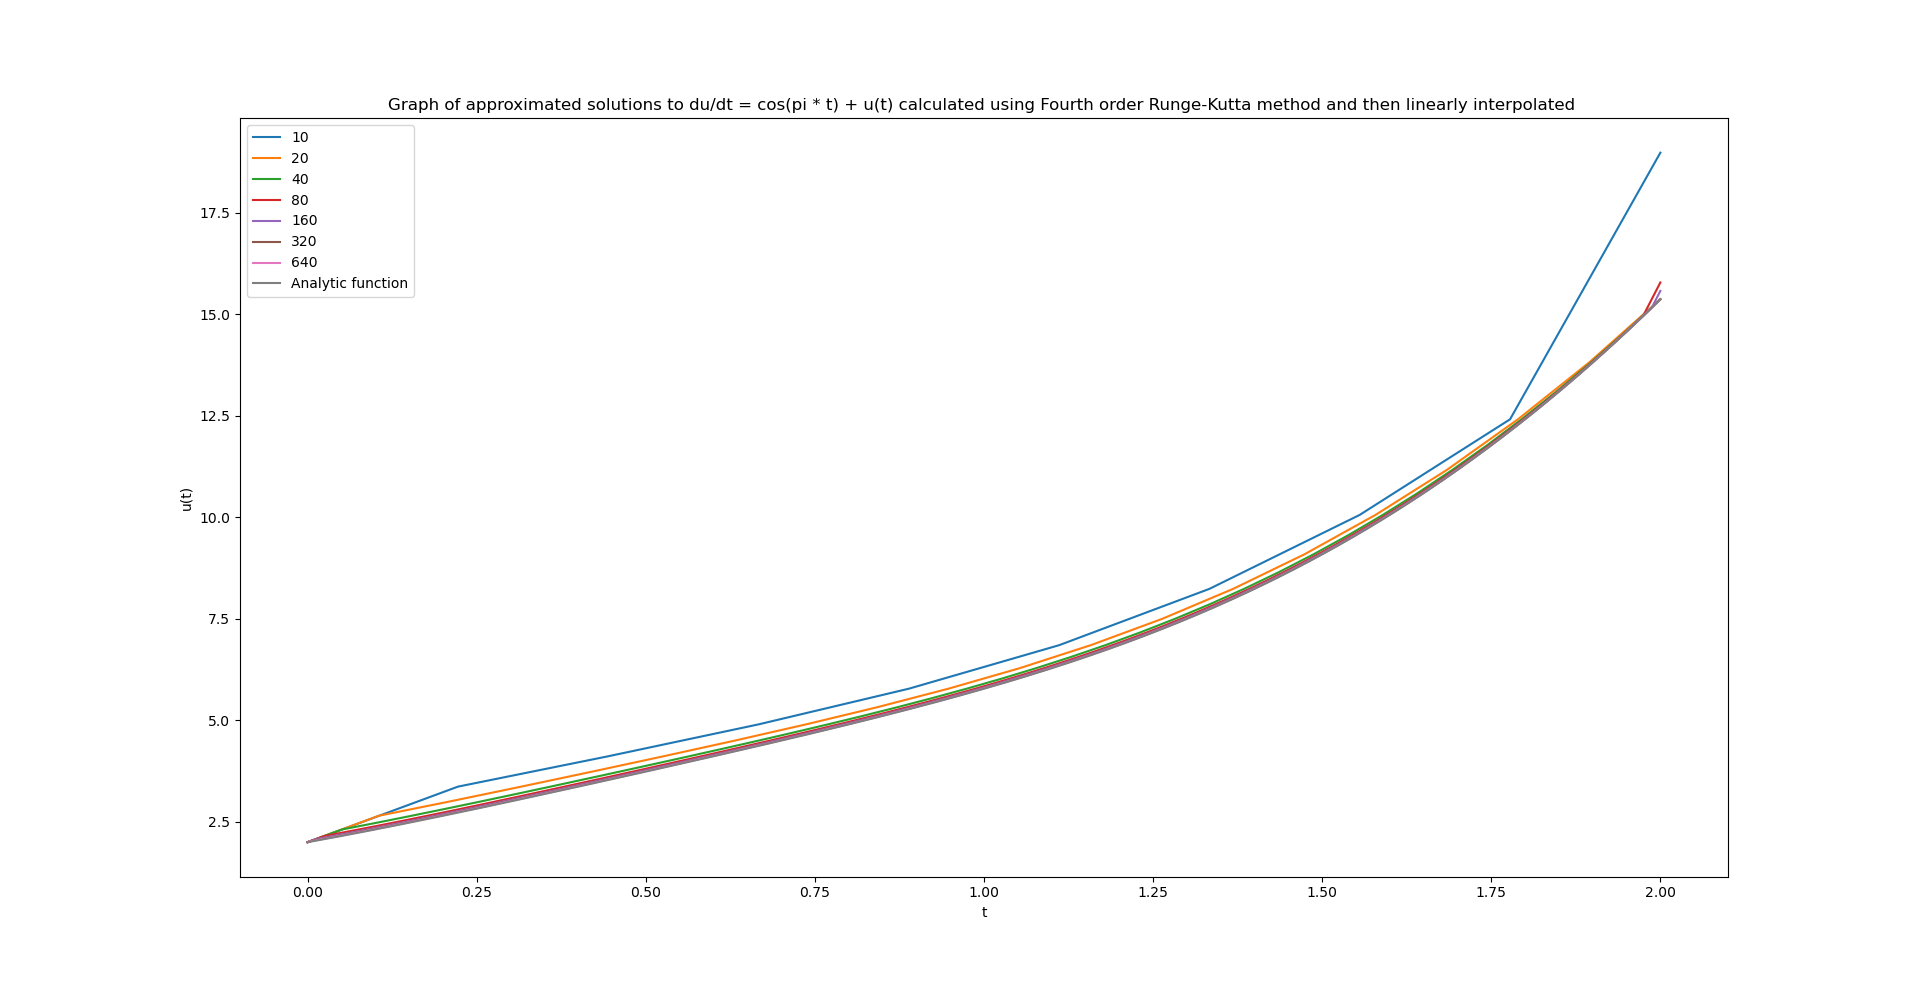
\includegraphics[angle=0,height=10cm]{./img/runge_4_function.png}
\end{center}

\begin{center}
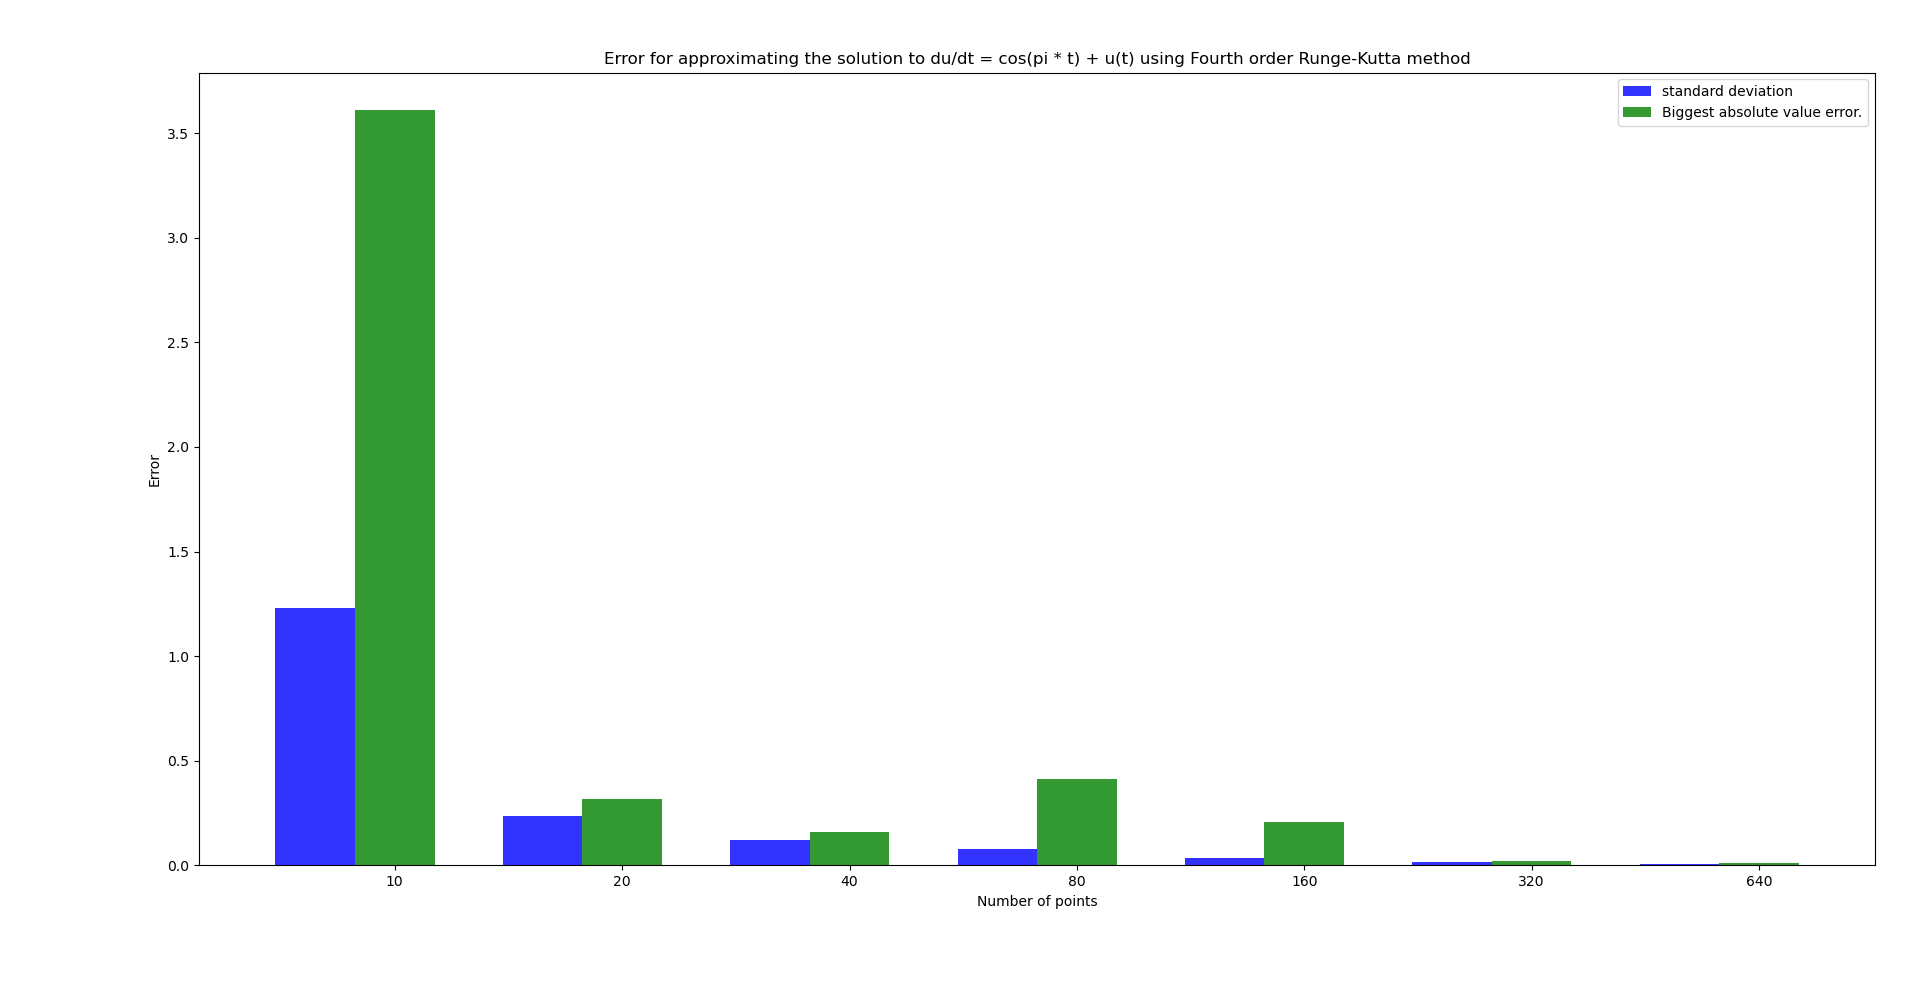
\includegraphics[angle=0,height=10cm]{./img/runge_4_error.png}
\end{center}




\subsection{Adam-Bashforth method}
\label{sec:orgdd9a132}

\begin{center}
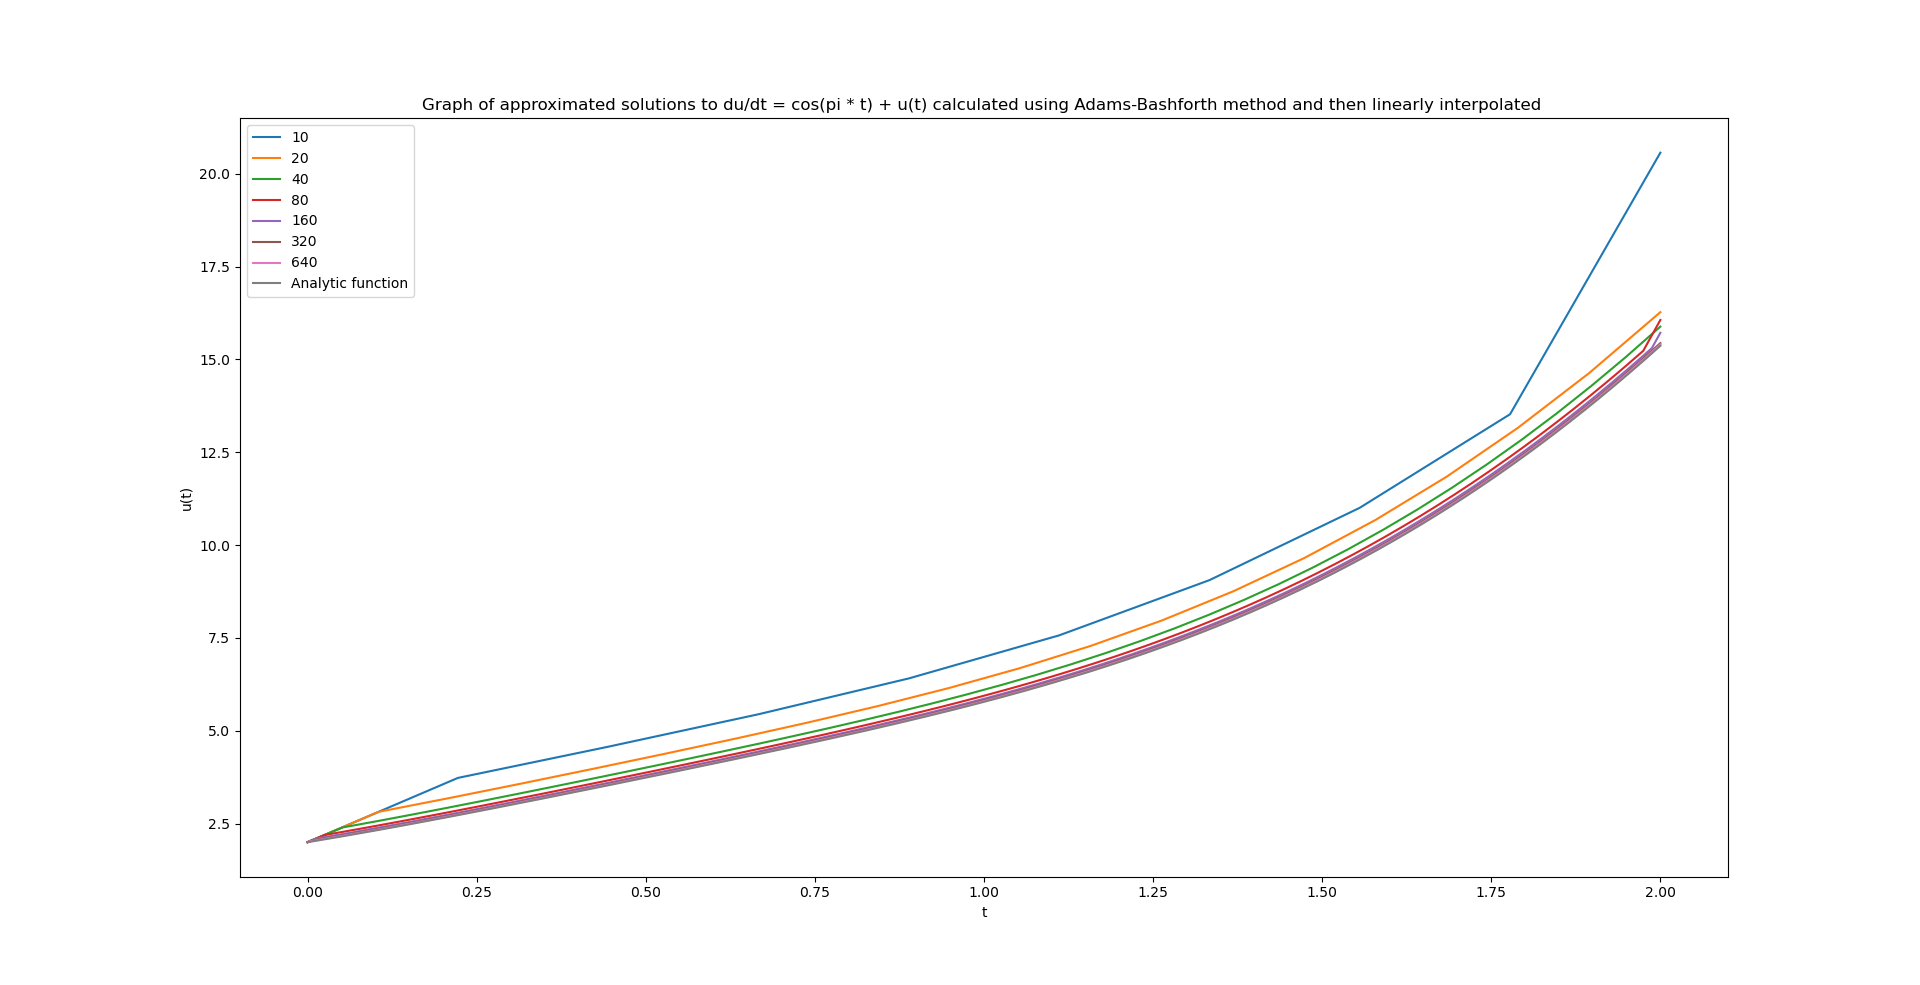
\includegraphics[angle=0,height=10cm]{./img/adam_function.png}
\end{center}

\begin{center}
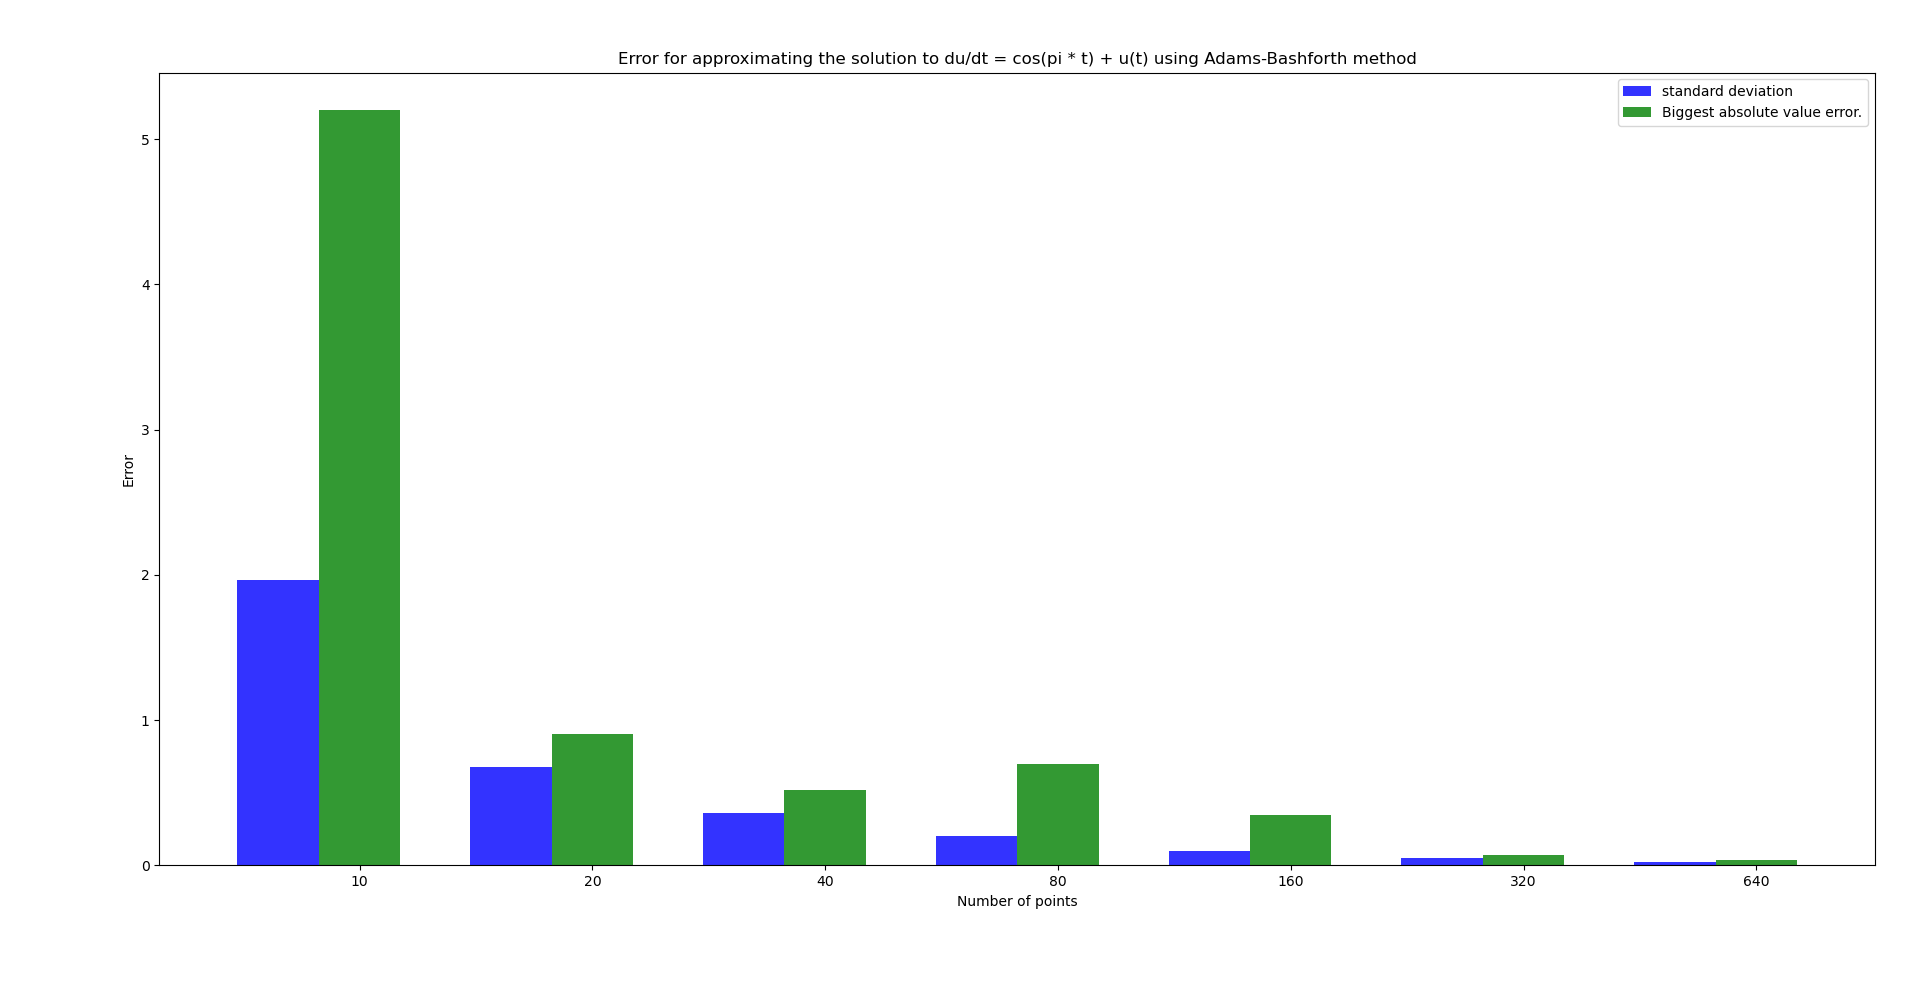
\includegraphics[angle=0,height=10cm]{./img/adam_error.png}
\end{center}

\section{Discussion}
\label{sec:orgba155ff}

As expected more points for all methods yields more accurate results, both
regarding average accuracy and minimizing the range of the error. We can see that
compared to Euler's method, the other methods converge quicker. And this makes sense
as the euler method's step forward depends on the the slope ahead being the same incline or
descent (derivative), as at the current point. The other methods uses the
derivative around the point in order for the step forward to be more accurate rather
than stepping forward relying on the slope ahead having constant derivative.

Comparing the Runge-Kutta methods and the Adam-Bashforth method yield no drastic difference. The
Adam-Bashforth method implemented in the code uses two steps, so it can be optimized with higher steps. This version of Adam-Bashforth also doesn't use a predictor, so using a multistep
method that uses a predictor, would probably be better than the predictor itself. For example by using the Moulton method with some Runge-Kutta would most definetly yield better results than
the Runge-Kutta method by itself.

Across the methods we also se that the ratio between average accuracy and range of error seems
to be the same for all methods. This perhaps relies more on the function itself, as for example
a function that has oscilating features when zoomed in will greatly affect this ratio. 
\end{document}
